\documentclass[12pt]{article}

\usepackage[utf8]{inputenc}
\usepackage[russian]{babel}
\usepackage{amsmath}
\usepackage{amsfonts}
\usepackage{geometry}
\usepackage{hyperref}
\usepackage{graphicx}
\usepackage{enumitem}
\usepackage[ruled,vlined]{algorithm2e}
\geometry{a4paper, margin=1in}
\usepackage{svg}
\usepackage{tikz}
\usetikzlibrary{arrows.meta, positioning}
\title{Безопасность квантовых вычислений \\ \large  }
\author{Голубович Тимур Б01-110}
\date{\today}

\begin{document}

\maketitle

\tableofcontents
\newpage

\section{Введение}

Безопасность квантовых вычислений становится критически важной из-за угроз, которые представляют квантовые технологии для традиционных методов защиты информации. С увеличением вычислительных мощностей квантовые компьютеры смогут эффективно факторизовать большие числа с помощью алгоритма Шора, что ставит под сомнение надежность криптографических алгоритмов, таких как RSA.

В ответ разрабатываются новые методы защиты, включая квантовое распределение ключей (QKD) и постквантовые криптографические алгоритмы, устойчивые к квантовым атакам. Эти технологии необходимы для обеспечения безопасности данных в будущем.

Таким образом, комплексный подход к безопасности квантовых вычислений, учитывающий технические аспекты, становится важным для специалистов в области информационной безопасности.

\vspace{1cm} % Adjust the space as needed

\begin{figure}[h] % Use figure environment for captions
    \centering
    \begin{tikzpicture}[
        % Style for first and second level nodes
        level 1/.style={draw, fill=blue!20, rectangle, minimum width=2cm, minimum height=1cm, align=center},
        level 2/.style={draw, fill=cyan!20, rectangle, minimum width=2cm, minimum height=1cm, align=center},
        % Style for third and fourth level nodes
        level 3/.style={draw, fill=red!20, rectangle, minimum width=2cm, minimum height=1cm, align=center},
        level 4/.style={draw, fill=orange!20, rectangle, minimum width=2cm, minimum height=1cm, align=center},
        arrow/.style={-{Stealth[scale=1.0]}, thick},
        node distance=0.8cm
    ]
    
    % Level 1 nodes
    \node[level 1] at (4, 0) (symmetric) {Симметричные\\ криптосхемы};
    \node[level 1] at (10, 0) (asymmetric) {Ассиметричные\\ криптосхемы};
    
    % Level 2 nodes
    \node[level 2] at (0, -2) (modern) {Современная\\ криптография};
    \node[level 2] at (3, -2) (block) {Блочные\\ шифры};
    \node[level 2] at (5.5, -2) (hash) {Хэш\\Функции};
    \node[level 2] at (8, -2) (digital) {Цифровая\\ подпись};
    \node[level 2] at (10.5, -2) (encryption) {С открытым\\ ключом};
    \node[level 2] at (13.5, -2) (key) {Распределение\\ ключа};
    
    % Level 3 nodes
    \node[level 3] at (0, -4) (attack) {Квантовая\\ атака};
    \node[level 3] at (3, -4) (grover) {Алгоритм\\ Гровера};
    \node[level 3] at (5.5, -4) (fft) {ВНТ};
    \node[level 3] at (10.5, -4) (shor) {Алгоритм\\ Шора};
    
    % Level 4 nodes
    \node[level 4] at (4, -6) (protection) {Для защиты достаточно\\ увеличить размер параметров};
    \node[level 4] at (11, -6) (vulnerability) {Криптосхемы будут взломаны,\\ увеличение параметров не помогает};
    
    % Drawing arrows for level 1 to level 2
    \draw[arrow] (symmetric.south) -- (block.north);
    \draw[arrow] (symmetric.south) -- (hash.north);
    
    \draw[arrow] (asymmetric.south) -- (digital.north);
    \draw[arrow] (asymmetric.south) -- (encryption.north);
    \draw[arrow] (asymmetric.south) -- (key.north);
    
    % Drawing arrows for level 4
    \draw[arrow] (protection.north) -- (grover.south);
    \draw[arrow] (protection.north) -- (fft.south);
    \draw[arrow] (vulnerability.north) -- (shor.south);
    
    % Additional arrows connecting level 3 to level 2
    \draw[arrow] (grover.north) -- (block.south);
    \draw[arrow] (fft.north) -- (hash.south);
    \draw[arrow] (shor.north) -- (digital.south);
    \draw[arrow] (shor.north) -- (encryption.south);
    \draw[arrow] (shor.north) -- (key.south);
    \end{tikzpicture}
\caption{Постквантовые криптографические механизмы}
\label{fig:post-mechs}
\end{figure}

\section{Квантовые алгоритмы и криптография}

Квантовые компьютеры могут угрожать традиционной криптографии. Например, алгоритм Шора позволяет эффективно факторизовать большие числа, что ставит под угрозу безопасность систем, основанных на RSA и других алгоритмах, использующих факторизацию. Это означает, что данные, защищенные с помощью таких методов, могут быть уязвимы к атакам с использованием квантовых компьютеров. Давайте подробней рассмотрим, как он работает.

\newpage

\subsection{Факторизация целых чисел}

Для начала, факторизация натурального числа есть его разложение в произведение простых множителей. Существование и единственность (с точностью до порядка следования множителей) такого разложения следует из основной теоремы арифметики. Очевидный алгоритм разложения числа на простые множители такой:

\begin{figure}[h]
    \centering
    \begin{algorithm}[H]
    \caption{Факторизация на классическом компьютере}
    \KwIn{число $ n \in \mathbb{N}$, которое необходимо факторизовать}
    \KwOut{первый простой делитель $d$}
    \State $ N \gets [\log_{2} n] + 1 $
    \Comment{Количество символов в двоичном представлении}
    
    \If{$n$ простое}{
        \KwRet{$n$} \Comment{Факторизация не требуется}
    }
    \For{каждое $a$ от $2$ до $\sqrt{n}$}{
        \If{$n \mod a = 0$}{
            \State $ d \gets a $ \Comment{Находим первый простой делитель}
            \KwRet{$d$}
        }
    }
    \end{algorithm}
    \caption{Примитивный алгоритм факторизации целового числа}
    \label{fig:algo1}
\end{figure}

Вопрос о существовании алгоритма факторизации с полиномиальной сложностью на классическом компьютере является одной из важных открытых проблем современной теории чисел. В то же время факторизация с полиномиальной сложностью возможна на квантовом компьютере с помощью алгоритма Шора (класс BQP).

\begin{figure}[h]
    \centering
    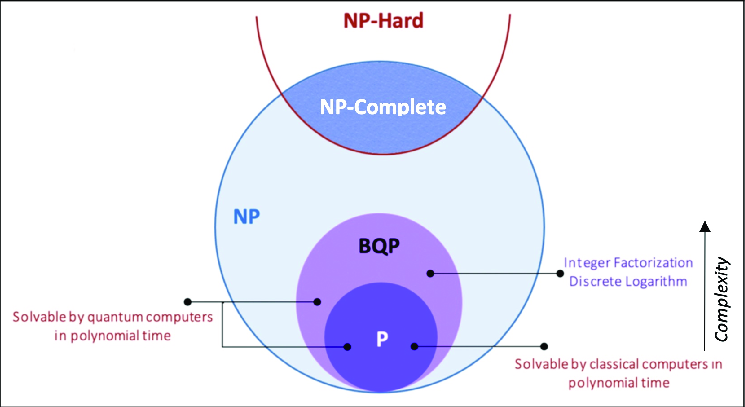
\includegraphics[width=\textwidth]{res/problems-complexity.png}
    \caption{Предположительная сложность задачи факторизации}
    \label{fig:compl}
\end{figure}

\newpage

\subsection{Алгоритм Шора}

Алгоритм Шора позволяет выполнить решение задачи факторизации за полиномиальное время. Это осуществляется за счет использования свойства квантового параллелизма и сведения задачи к поиску периода функции.

Допустим, нам необходимо разложить на множители некоторое число \( N \). Изначально выберем произвольное число \( a < N \) и рассмотрим функцию \( f_a(x) = a^x \mod N \).

Функция \( f_a(x) \) является периодической с периодом \( r \). Период \( r \) является порядком числа \( a \): \( a^r \equiv 1 \mod N \) и \( \forall i < r \Rightarrow a^i \not\equiv 1 \mod N \). Если число \( N \) простое, то период \( r \) будет равен \( N - 1 \). Этот случай весьма простой и легко реализуется проверкой на простоту классическими методами. В общем случае \( f_a(x + r) = f_a(x) \). Если период \( r \) известен, то разложение на множители числа \( N \) легко можно определить классическими методами. В частности, если период \( r \) является четным числом, то из соотношения \( a^r - 1 \equiv 0 \mod N \) можно записать:

\[
(a^{r/2} - 1)(a^{r/2} + 1) \equiv 0 \mod N
\]

Так как \((a^{r/2} - 1)(a^{r/2} + 1)\) делится на \( N \), то оба сомножителя имеют общие с \( N \) делители. Эти делители можно определить классическим алгоритмом Евклида по поиску наибольшего общего делителя. Если же период \( r \) является нечетным или \((a^{r/2} - 1)(a^{r/2} + 1)\) вырождается в ноль, то следует выбрать другое число \( a \). Для больших чисел \( N \) это случается редко.

Квантовый алгоритм Шора предназначен для быстрого поиска периода \( r \). Для реализации алгоритма необходимо использовать квантовый компьютер с двумя квантовыми регистрами размера \( n \). Причем размер должен быть таким, что \( M = 2^n > N \), \( M \approx N^2 \).

\begin{figure}[h]
    \centering
    \begin{algorithm}[H]
    \caption{Алгоритм Шора для факторизации числа \( N \)}
    \KwIn{Целое число \( N \) для факторизации}
    \KwOut{Непростые множители числа \( N \)}
    \While{не найден делитель}{
        Выбрать случайное число \( a \) такое, что \( 1 < a < N \)\\
        \If{gcd(\( a, N \)) \neq 1}{
            \KwRet{gcd(\( a, N \))} \Comment{Найден делитель}
        }
        \( r \gets \text{find\_period}(a, N) \) \Comment{Квантовый алгоритм для нахождения периода}

        \If{r нечетный \textbf{или} \( a^{r/2} \equiv -1 \mod N \)}{
            \KwContinue \Comment{Период не подходит, продолжаем с другим \( a \)}
        }
        \( x_1 \gets a^{r/2} \mod N \)\\
        \( x_2 \gets N - x_1 \)\\
        \If{gcd(\( x_1, N \)) \neq 1}{
            \KwRet{gcd(\( x_1, N \))} \Comment{Возвращаем делители}
        }
        \If{gcd(\( x_2, N \)) \neq 1}{
            \KwRet{gcd(\( x_2, N \))} \Comment{Возвращаем делители}
        }
    }
    \KwRet{Не удалось найти делители} \Comment{Если делители не найдены}
    \end{algorithm}
    \caption{Алгоритм Шора}
    \label{fig:post-mechs}
\end{figure}

\newpage

\subsection{Квантовый отжиг}

Квантовый отжиг (\textit{Quantum Annealing}) — это метод решения оптимизационных задач, который использует квантовые эффекты для поиска низкоэнергетических состояний системы. Он основан на классическом отжиге, где система охлаждается для достижения минимальной энергии, но в отличие от классического подхода, квантовый отжиг применяет суперпозицию и туннелирование, что позволяет избегать локальных минимумов. Процесс включает в себя несколько этапов:

\begin{figure}[h]
    \centering
    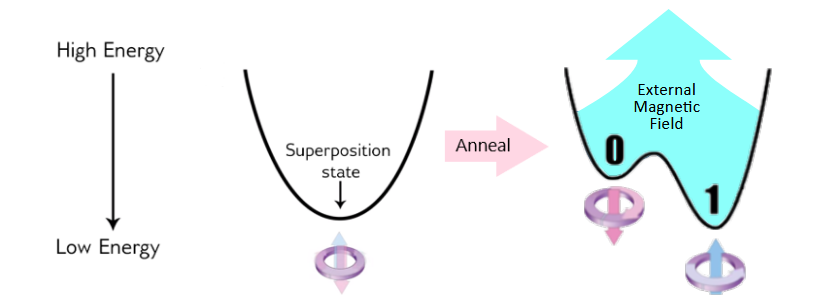
\includegraphics[width=\textwidth]{res/evolution.png}
    \caption{Энергетическая диаграмма процесса отжига}
    \label{fig:compl}
\end{figure}

\begin{enumerate}
    \item \textbf{Инициализация}: Кубит есть основная единица квантовой информации в квантовом процессоре $D-Wave (QPU)$. Он может находиться в состоянии 0, 1 или одновременно в обоих состояниях (суперпозиция). Система начинается с кубитов в состоянии суперпозиции, соответствующем одному минимуму энергии.
    
    \item \textbf{Энергетический ландшафт}: По мере эволюции процесса отжига энергетический ландшафт изменяется, создавая множество минимумов. Цель состоит в том, чтобы направить систему к состоянию с наименьшей энергией.
    
    \item \textbf{Процесс отжига}: Система переходит от начального гамильтониана к конечному гамильтониану, стремясь оставаться в состоянии с наименьшей энергией на протяжении всего процесса.
    
    \item \textbf{Измерение}: В конце процесса отжига каждый кубит оказывается в классическом состоянии (0 или 1), представляя решение задачи.
\end{enumerate}

Квантовый отжиг находит применение в различных областях, таких как комбинаторные задачи оптимизации, машинное обучение и логистика. Технологии, такие как квантовые процессоры от \textit{D-Wave}, специально разработаны для работы с такими задачами. Несмотря на то, что квантовый отжиг находится на ранних стадиях развития, он уже демонстрирует многообещающие результаты в решении сложных оптимизационных задач. Таким образом он представляет угрозу для симметричной криптографии, особенно для потоковых шифров. Существуют шифры, устойчивые к классическим атакам, но они уязвимы к квантовому отжигу. Среди них находится Grain-128a, основная схема финалиста NIST Lightweight Cryptography Grain-128AEAD. Стандартизированные шифры широко используются как в военной, так и в гражданской отраслях. Стандартизация шифра с такой уязвимостью позволит внедрить угрозу во многие сектора:

\begin{itemize}[label=--]
    \item обработка секретных данных;
    \item устройства Интернета вещей;
    \item телекоммуникации.
\end{itemize}

Задачи для квантового отжига формулируются в виде \textbf{QUBO} или \textbf{Ising} модели. Рассмотрим задачу QUBO. 

\subsection{QUBO}

\textbf{Определение:} QUBO (Quadratic Unconstrained Binary Optimization) — это задача оптимизации, в которой необходимо найти бинарный вектор \( x \) (состоящий из 0 и 1), минимизирующий квадратичную функцию. Формально задача может быть записана как:

\begin{align*}
\min_{x \in \{0, 1\}^n} f(x) = x^T Q x 
\end{align*}

где \( Q \) — симметричная матрица, а \( x \) — бинарный вектор.

\textbf{Основные характеристики:}
\begin{itemize}
    \item \textbf{Бинарные переменные:} Переменные \( x_i \) могут принимать значения только 0 или 1.
    \item \textbf{Квадратичная функция:} Целевая функция состоит из линейных и квадратных членов.
    \item \textbf{Решение:} Задачи решаются классическими (методы ветвей и границ, генетические алгоритмы) и квантовыми алгоритмами (например, квантовым отжигом).
\end{itemize}

\newpage

\section{Устойчивость к квантовым атакам}

Устойчивость к квантовым атакам — это важная тема в области криптографии, особенно с учетом развития квантовых компьютеров, которые могут угрожать традиционным криптографическим алгоритмам. Квантовые компьютеры обладают способностью решать определенные задачи гораздо быстрее, чем классические компьютеры. Это означает, что если квантовые компьютеры достигнут достаточной мощности, они смогут легко взломать многие существующие криптографические схемы.

\subsection{Постквантовая криптография}
В ответ на эту угрозу разрабатываются новые криптографические алгоритмы, которые устойчивы к квантовым атакам. Эти алгоритмы называются постквантовыми и включают в себя:

\begin{enumerate}[label=\arabic*.]
    \item \textbf{Криптография на основе решеток:} Алгоритмы, основанные на математических структурах, называемых решетками, считаются одними из самых перспективных для создания устойчивых к квантовым атакам систем. Примеры включают схемы шифрования NTRU и схемы цифровой подписи на основе решеток.
    
    \item \textbf{Криптография на основе многочленов:} Использует задачи, связанные с многочленами, которые трудно решать даже для квантовых компьютеров. 
    
    \item \textbf{Криптография на основе кодов:} Алгоритмы, использующие ошибки коррекции кодов, также рассматриваются как потенциально устойчивые к квантовым атакам. Примером является система McEliece.
\end{enumerate}

\subsection{Квантовые алгоритмы}
Квантовые алгоритмы продолжают развиваться, и помимо алгоритма Шора, стоит упомянуть:

\begin{itemize}
    \item \textbf{Алгоритм Гровера:} Этот алгоритм позволяет ускорить поиск в неупорядоченной базе данных, находя элемент в базе данных из $N$ элементов за $O(\sqrt{N})$ времени.
    
    \item \textbf{Квантовые алгоритмы для симуляции квантовых систем:} Эти алгоритмы позволяют моделировать квантовые системы и процессы, что может быть полезно в химии, физике и других областях.
    
    \item \textbf{Квантовые алгоритмы для оптимизации:} Разрабатываются алгоритмы, которые используют квантовые свойства для решения задач оптимизации, такие как алгоритмы QAOA (Quantum Approximate Optimization Algorithm).
\end{itemize}

\newpage

\section{Заключение}

В заключение, развитие квантовых технологий представляет собой процесс, который одновременно открывает новые горизонты и создает угрозы для существующих систем безопасности. Квантовые алгоритмы, такие как алгоритм Шора или алгоритм квантового отжига, демонстрируют, что традиционные методы криптографии, основанные на факторизации или оптимизационных задачах, могут оказаться уязвимыми в условиях появления мощных квантовых компьютеров. В ответ на эти вызовы развивается квантовая криптография.

Тем не менее, на данный момент мощности квантовых компьютеров все еще остаются ограниченными, что дает время для исследования и разработки новых постквантовых криптографических алгоритмов, способных защитить данные от потенциальных квантовых атак. Это создает надежду на то, что мы сможем адаптироваться к изменениям в области вычислительных технологий и сохранить безопасность цифровых коммуникаций в будущем. Важно продолжать инвестировать в исследования и разработки в этой области, чтобы обеспечить защиту данных в эпоху квантовых вычислений. 

\begin{thebibliography}{6}
    \bibitem{shor_is_threat} \href{https://www.quantamagazine.org/thirty-years-later-a-speed-boost-for-quantum-factoring-20231017/}{Thirty Years Later, a Speed Boost for Quantum Factoring}

    \bibitem{postquantum} \href{https://www.gazprombank.tech/blog/694}{Постквантовый переход}
    
    \bibitem{factorization} \href{https://www.theoremoftheday.org/MathsStudyGroup/ADF37A.pdf}{Factorization of Integers}
    
    \bibitem{shors_algorithm} \href{https://qsim.tsu.ru/lectures/Shor's_algorithm}{Алгоритм Шора} 

    \bibitem{qubo} \href{https://wigner.hu/~koniorczykmatyas/qubo/literature/1811.11538.pdf}{A Tutorial on Formulating and Using QUBO Models}

    \bibitem{anneal} \href{https://docs.dwavesys.com/docs/latest/c_gs_2.html}{What is Quantum Annealing?}

    \bibitem{anneal1} \href{https://sd-magazine.eu/index.php/sd/article/download/216/167/}{The possible impact of quantum annealing on cybersecurity}

    \bibitem{anneal2} \href{https://nattothoughts.substack.com/p/chinas-quantum-tunneling-breakthrough}{Quantum tunneling breakthrough}

    \bibitem{qthreat} \href{https://qapp.tech/help/quantum-threat}{Квантовая атака}

    \bibitem{qsecurity} \href{https://www.ptsecurity.com/ru-ru/research/analytics/bezopasnost-kvantovyh-technologiy-v-sphere-it/}{Безопасность квантовых технологий в сфере IT}

\end{thebibliography}

\end{document}